\definecolor{zzttqq}{rgb}{0.15,0.35,0.15}

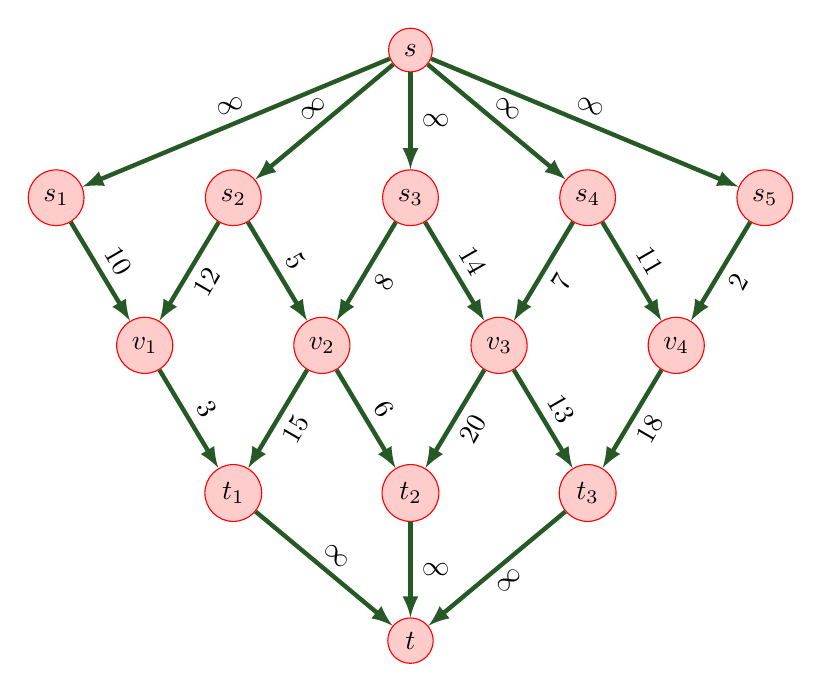
\begin{tikzpicture}[x=1.5cm, y=1.5cm]
	\node[circle,draw=red,fill=red!20] (s) at (0,4.25) {$s$};
	\node[circle,draw=red,fill=red!20] (s1) at (-3,3) {$s_1$};
	\node[circle,draw=red,fill=red!20] (s2) at (-1.5,3) {$s_2$};
	\node[circle,draw=red,fill=red!20] (s3) at (0,3) {$s_3$};
	\node[circle,draw=red,fill=red!20] (s4) at (1.5,3) {$s_4$};
	\node[circle,draw=red,fill=red!20] (s5) at (3,3) {$s_5$};
    \node[circle,draw=red,fill=red!20!] (v1) at (-2.25,1.75) {$v_1$};
    \node[circle,draw=red,fill=red!20!] (v2) at (-0.75,1.75) {$v_2$};
    \node[circle,draw=red,fill=red!20!] (v3) at (0.75,1.75) {$v_3$};
    \node[circle,draw=red,fill=red!20!] (v4) at (2.25,1.75) {$v_4$};
    \node[circle,draw=red,fill=red!20!] (t1) at (-1.5,0.5) {$t_1$};
    \node[circle,draw=red,fill=red!20!] (t2) at (0,0.5) {$t_2$};
    \node[circle,draw=red,fill=red!20!] (t3) at (1.5,0.5) {$t_3$};
    \node[circle,draw=red,fill=red!20!] (t) at (0,-0.75) {$t$};
    
	\draw[color=zzttqq, ultra thick, -latex]  (s) edge node[rotate = 20, above,color=black]{$\infty$} (s1);
	\draw[color=zzttqq, ultra thick, -latex]  (s) edge node[rotate = 40, above,color=black]{$\infty$} (s2);   
	\draw[color=zzttqq, ultra thick, -latex]  (s) edge node[right,color=black]{$\infty$} (s3);			
	\draw[color=zzttqq, ultra thick, -latex]  (s) edge node[rotate = -40, above,color=black]{$\infty$} (s4);
	\draw[color=zzttqq, ultra thick, -latex]  (s) edge node[rotate = -20, above,color=black]{$\infty$} (s5);
	
    \draw[color=zzttqq, ultra thick, -latex]  (s1) edge node[rotate = -60, above,color=black]{10} (v1);
    \draw[color=zzttqq, ultra thick, -latex]  (s2) edge node[rotate = 60, below,color=black]{12} (v1);
    \draw[color=zzttqq, ultra thick, -latex]  (s2) edge node[rotate = -60, above,color=black]{5} (v2);
    \draw[color=zzttqq, ultra thick, -latex]  (s3) edge node[rotate = 60, below,color=black]{8} (v2);
    \draw[color=zzttqq, ultra thick, -latex]  (s3) edge node[rotate = -60, above,color=black]{14} (v3);
    \draw[color=zzttqq, ultra thick, -latex]  (s4) edge node[rotate = 60, below,color=black]{7} (v3);
    \draw[color=zzttqq, ultra thick, -latex]  (s4) edge node[rotate = -60, above,color=black]{11} (v4);
    \draw[color=zzttqq, ultra thick, -latex]  (s5) edge node[rotate = 60, below,color=black]{2} (v4);
	
	\draw[color=zzttqq, ultra thick, -latex]  (v1) edge node[rotate = -60, above,color=black]{3} (t1);
    \draw[color=zzttqq, ultra thick, -latex]  (v2) edge node[rotate = 60, below,color=black]{15} (t1);
    \draw[color=zzttqq, ultra thick, -latex]  (v2) edge node[rotate = -60, above,color=black]{6} (t2);
    \draw[color=zzttqq, ultra thick, -latex]  (v3) edge node[rotate = 60, below,color=black]{20} (t2);
    \draw[color=zzttqq, ultra thick, -latex]  (v3) edge node[rotate = -60, above,color=black]{13} (t3);
    \draw[color=zzttqq, ultra thick, -latex]  (v4) edge node[rotate = 60, below,color=black]{18} (t3);
    
    \draw[color=zzttqq, ultra thick, -latex]  (t1) edge node[rotate = -45, above,color=black]{$\infty$} (t);
	\draw[color=zzttqq, ultra thick, -latex]  (t2) edge node[right,color=black]{$\infty$} (t);   
	\draw[color=zzttqq, ultra thick, -latex]  (t3) edge node[rotate = 45,below,color=black]{$\infty$} (t);	
	
\end{tikzpicture}